\section{Results}
\label{results}

Our Spark program is written in Scala using Hadoop distribution $2.7.2$, and run on a Intel (R) Xeon machine with two physical CPUs. Each CPU has $16$ E$5-2650$ @ $2.00$GHz cores, giving us a total $32$ cores. The machine also has $32$GB of RAM, and runs Ubuntu $16.04$.  

\subsection{Input description}

As discussed earlier, our input graph $G$ is an undirected, unweighted graph with $679965$ edges and $899162$ vertices. Each vertex and edge is represented using 8 bytes and so the total amount of memory required by our graph is about $20$MB. 

Our input graph also consists of $199004$ connected components, with the maximum component size at $145$ and the minimum at $2$. The distribution of component sizes is shown in Fig. \ref{fig:cs-overall}, where the numbers of components with sizes above, say $40$, were dwarfed by the components with smaller sizes. Fig. \ref{fig:cs-selected} is an alternative figure that reveals the distribution of larger components. 

To investigate the scalability of our code for increasing input, we replicate the graph by doubling it (labeled graph $G_2$) then quadrupling it (labeled graph $G_4$), whilst prerserving the same structure as far as connected components are concerned.

\subsection{Failures and connectivity loss analysis}

For each of the four scenarios described in Sec. \ref{methods}, we vary the number of threads and partitions, compute the percentage of loss, and plot this value against the number of nodes removed from the graph. In all the tables and figures below, $R$ corresponds to random failures, $D$ to degree based failures, $BC$ to betweenness centrality (load) failures, and $C$ to cascading failures. Fig. \ref{fig:loss-100} and \ref{fig:loss-1000} present a refined view demonstrating the progression of loss for the first 100 and 1000 failures on transmission and distribution nodes. Fig. \ref{fig:loss-all} shows the loss for the entire failures. The connectivity loss is faint and proportional to the number of failures in the random case. It is worse for the cascading scenario, whereas the connectivity losses associated with the load-based versus degree based scenarios are more or less comparable. These findings are confirmed in Table~\ref{resilience}, which presents, for each scenario, the percentage of failed nodes effecting in $60\%$ and $80\%$ (nearly total) connectivity loss. Some of these figures, particularly, the relatively high percentages required in each of the $BC$, $D$, and $R$ scenarios that precede total failure, can be interpreted to say that the Lebanese grid is highly redundant, and thus somehow resilient, thanks to its decomposition into numerous components and its reliance on local diesel generators that alleviate the effects of blackouts and failures. 


\begin{table}[t]
\centering
\caption{Percentage of vertices to be removed to reach $60\%$ and $80\%$ losses}
\label{tab:threshold-percentage}
{\small
\begin{tabular}{||c||c|c|c|c||}
\hline
\textbf{Loss}	&\cellcolor{black!10}BC&	\cellcolor{black!10}C & \cellcolor{black!10} R & \cellcolor{black!10} D \\ \hline \hline
60\% &		11.6\%&	4.3\%	&59.8\%&	7.7\%	 \\ \hline		
80\%	&		27.8\%&	14.6\%	&79.7\%&	29.5\%	 \\ \hline		
\end{tabular}
}
\label{resilience}
\end{table}




\begin{figure}
\centering
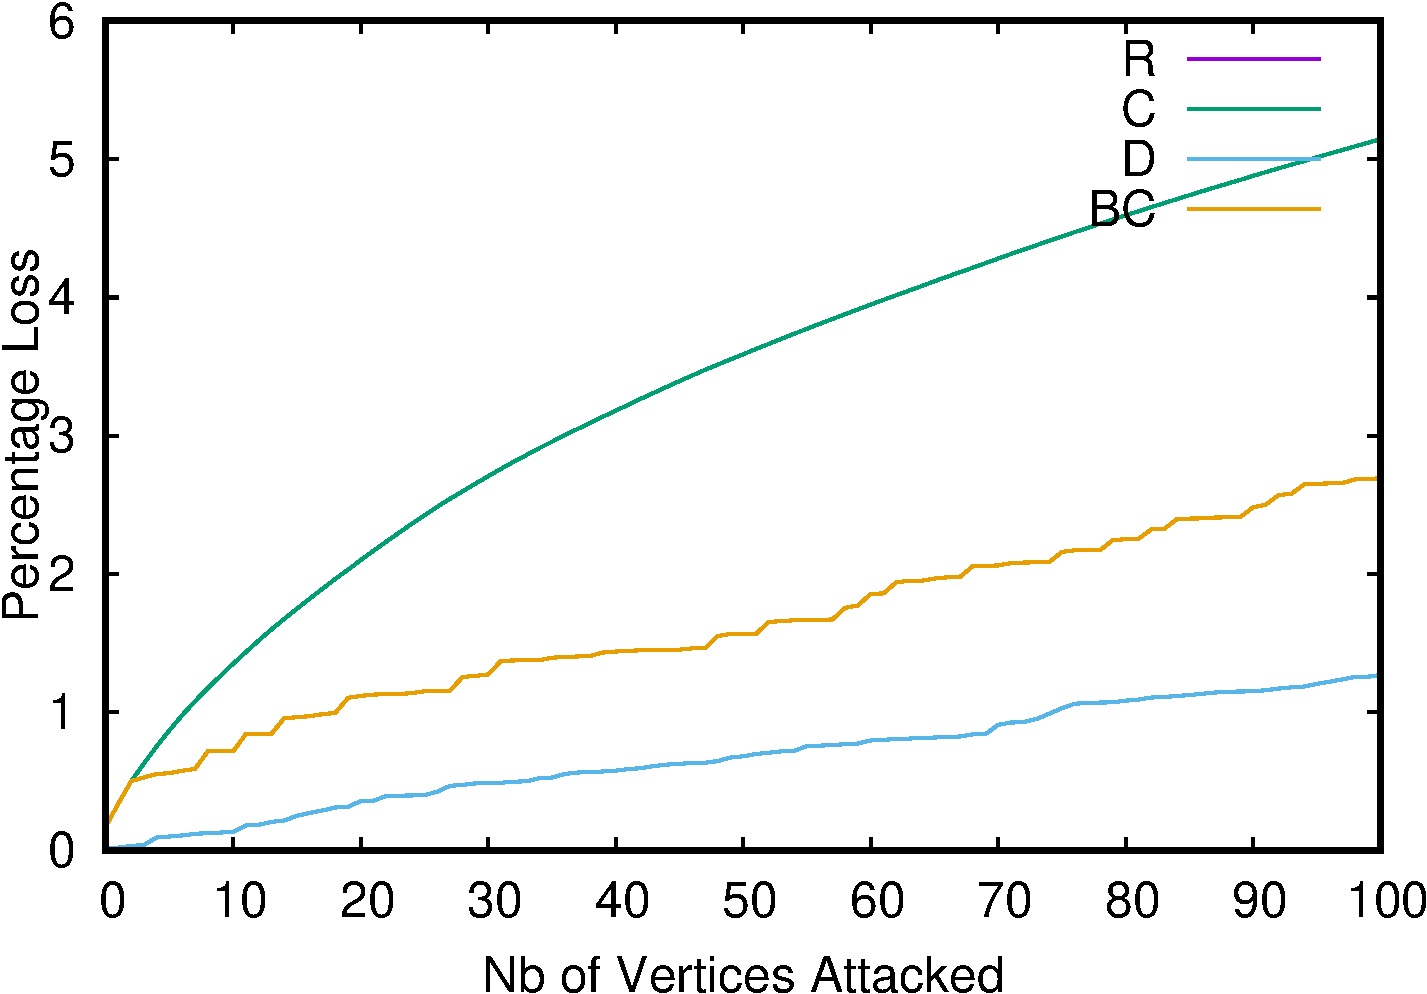
\includegraphics[scale=0.35]{bench/loss-100-crop.pdf}
\caption{Loss percentage: first 100 attacks}
\label{fig:loss-100}
\end{figure}

\begin{figure}
\centering
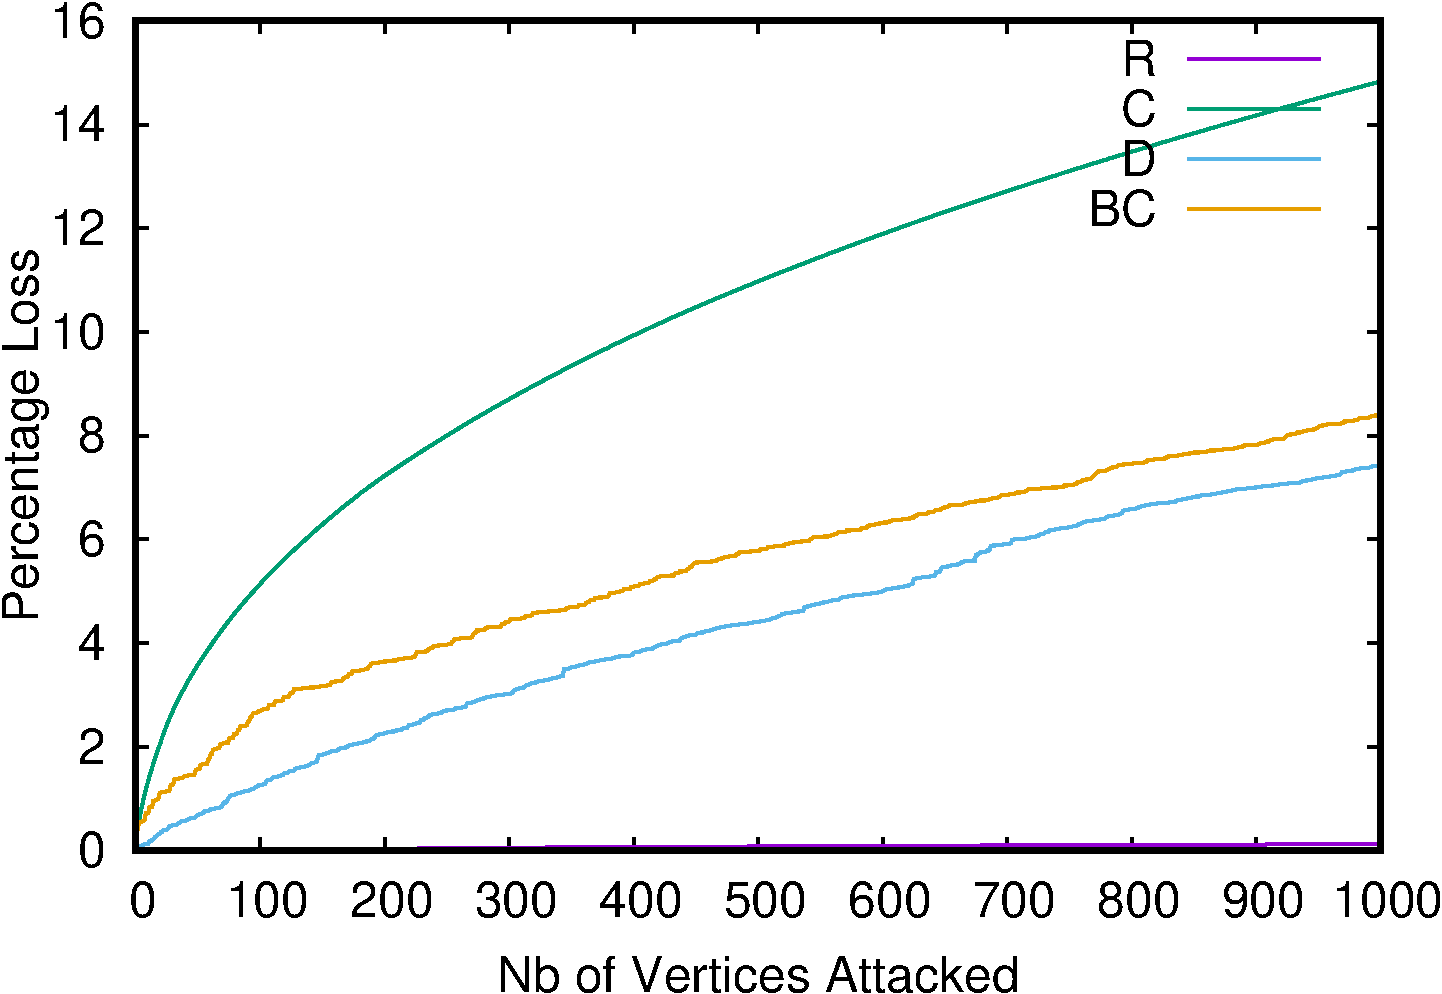
\includegraphics[scale=0.35]{bench/loss-1000-crop.pdf}
\caption{Loss percentage: first 1000 attacks}
\label{fig:loss-1000}
\end{figure}

\begin{figure}
\centering
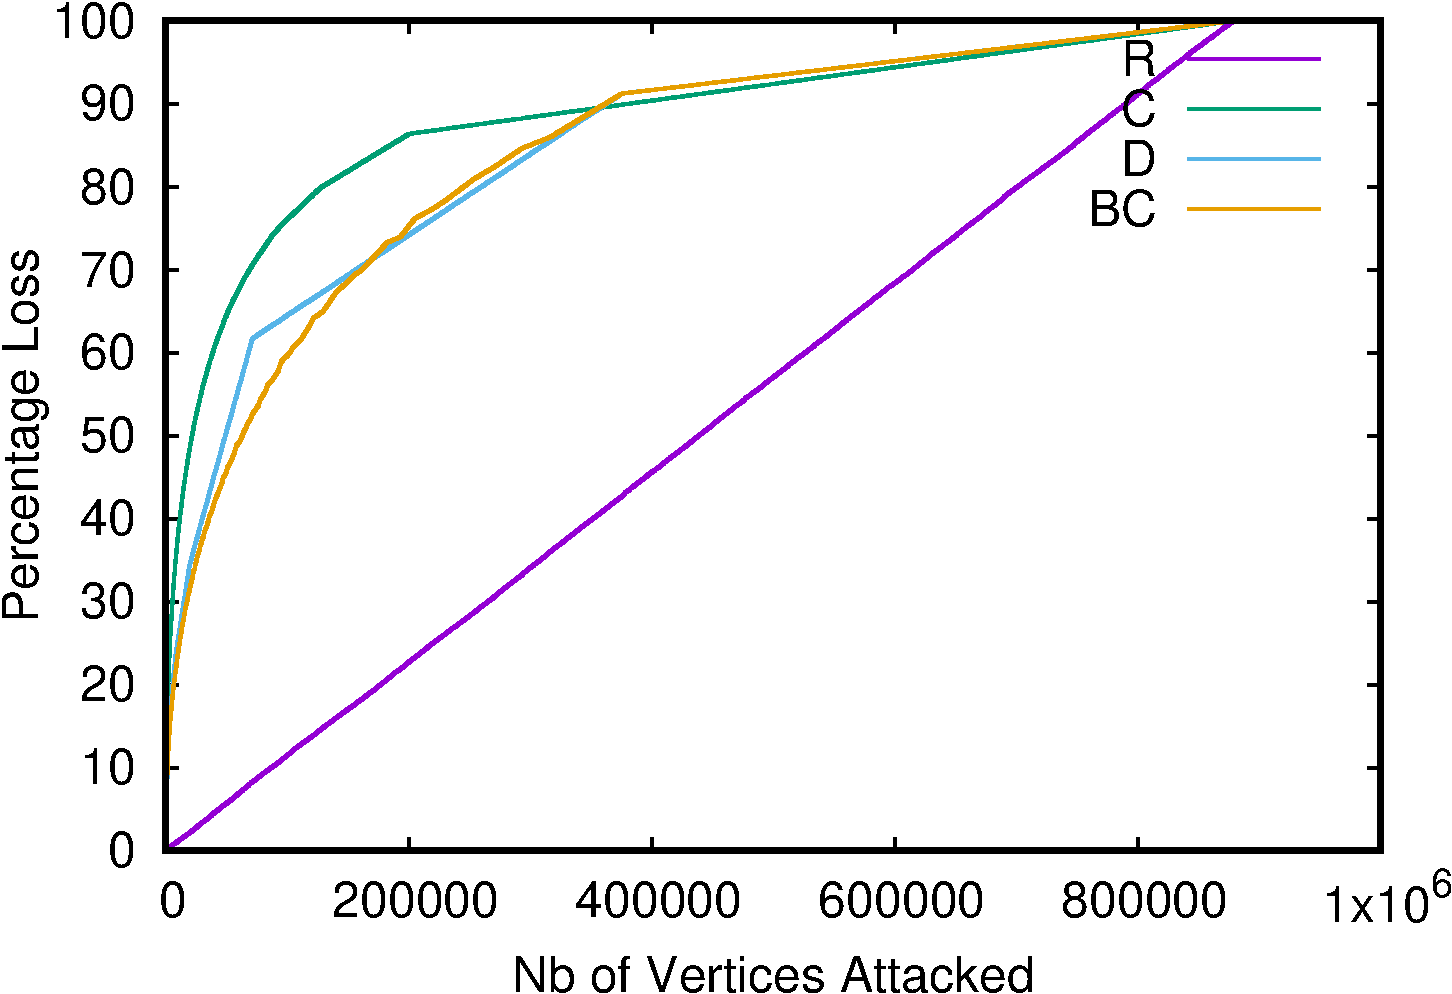
\includegraphics[scale=0.35]{bench/loss-all-crop.pdf}
\caption{Loss percentage: overall attacks}
\label{fig:loss-all}
\end{figure}

\subsection{Run-time and parallel efficiency analysis}
The run-time and parallel efficiency for each pair of ({\it thread},{\it partition}) values using our input graphs are shown in Table \ref{tab:graph1}, \ref{tab:graph2}, and \ref{tab:graph4}, for $G$, $G_2$, and $G_4$ respectively. 
%
\edited{
Here, parallel efficiency is defined as $\frac{T_s}{p\cdot T_p}$, where $T_s$ denotes the serial run-time and $T_p$ denotes the parallel run-time given $p$ parallel processes.}
%
The timings shown in the Tables correspond to the parallel phase of the algorithm. The sequential run-time was omitted because it was extremely negligible compared to the parallel part that is of higher order (in contrast to linear running time in steps 7 and 8).
%
By default, Spark sets the partition size at 64 MB. This is too large for our given graph. As a result, we choose to override the default value by specifying the number of partitions at compile time. When this is done, Spark re-adjusts the size of each partition based on their total number as well as on the size of the input graph. The several connected components in each graph get mapped onto all partitions such that the number of vertices in each partition is balanced across all partitions. We experiment with a number of partitions ranging from $4$, $8$, $16$, and $32$ in order to explore the effect that the number of partitions have on run-time and parallel efficiency. From Fig. \ref{fig:cs-overall} and \ref{fig:cs-selected}, we gather that there would be enough connected components in each partition to engage all threads assigned to the partition. Also, the fact that many connected components have sizes greater than, say, 40, ensures that the distributed work is more or less balanced.

As expected, for all three graphs, the fastest and yet the worst parallel efficiency correspond to the R (random failures) scenario that does not rely on any centrality measure computation. In contrast, the highest run-times and hence best efficiency are for the C (cascading scenario) that updates the betweenness centrality of all the nodes following each node removal. It is clear that the more work entailed by a certain scenario, the better it will be for the parallel program to compensate for the overheads associated with the partitioning and scheduling operations. Reading across the three tables for the same partition size and same scenario, our tool shows improved scalability as the input size grows. 

For each given graph and for each scenario employed, we notice that the actual run-time has opposing trends that depend on the number of partitions. For all three tables, there is a cut-off value for the number of partitions, before which run-time continues to improve, and after which it starts to deteriorate. For graph $G$, the cut-off number is at $8$, for graph $G_2$ it is somewhere between $8$ and $16$, and for $G_4$, it is at $16$. We justify the improvement in run-time as we move closer to the cut-off threshold as follows. With a higher number of partitions, one would expect that the multiple threads will be spread about, sharing the work but on data that is more split into distinct regions of main memory. As such, we have reduced contention over the shared address space, as well as scheduling costs associated with managing threads on one single partition. We now argue that creating more partitions beyond the cut-off number drastically affects the performance and introduces a huge overhead -- particularly when the number of threads is low. For instance, in Table II, if we consider only one thread of the BC scenario, it takes 161 (resp. 423) seconds in case of 4 (resp. 32) partitions. We attribute this overhead to the shuffling and repartition operations taking place at the end of each stage that assigns one or more threads from one partition to another. In that phase, some transformations (e.g., \texttt{groupByKey}, \texttt{reduceByKey}, \texttt{join} operations) require shuffling and repartitioning of data, for instance, to group all the items with the same keys in the same partition. 

With that said, we observe that efficiency actually improves for larger partitions. This isn't to be construed, however, to mean that the parallelisation has improved in any way, but rather that the rate of deterioration in the performance for a smaller number of threads (particularly, the case of one thread) is higher when the number of partitions exceeds the cut-off number, resulting in a higher-speedup as the number of threads grows larger. 

%Our own Spark implementation of contingency analysis executes in real-time for the entire power grid, achieving a speed-up of ? on ? processors. We conclude with a spatial understanding of the hotspots on Lebanese soil where energy centers can be exposed and are at risk, using a spatial correlation supported by a binary search tree. The amenability of our work to big data processing makes it extendable to larger networks of networks, towards a fuller understanding of resilence at many vital levels beyond the power grid. Examples are as communications network, Internet networks, transportation networks, hospitals and medical centers networks, to name a few.





\begin{figure}
\centering
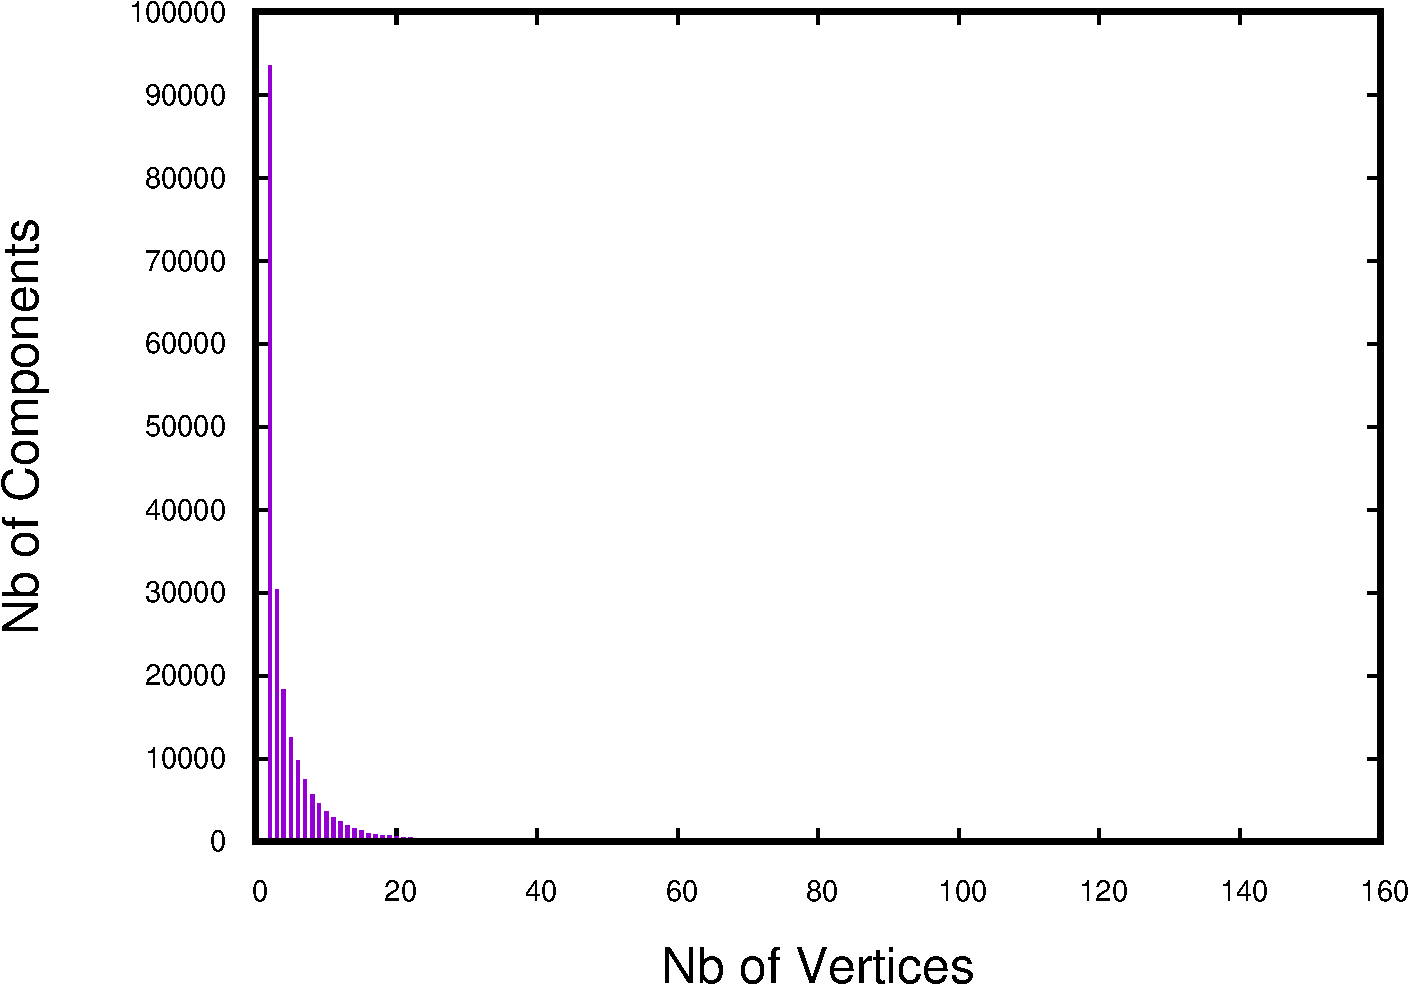
\includegraphics[scale=0.35]{bench/frequencyall-crop.pdf}
\caption{Components size -- overall distribution}
\label{fig:cs-overall}
\end{figure}

\begin{figure}
\centering
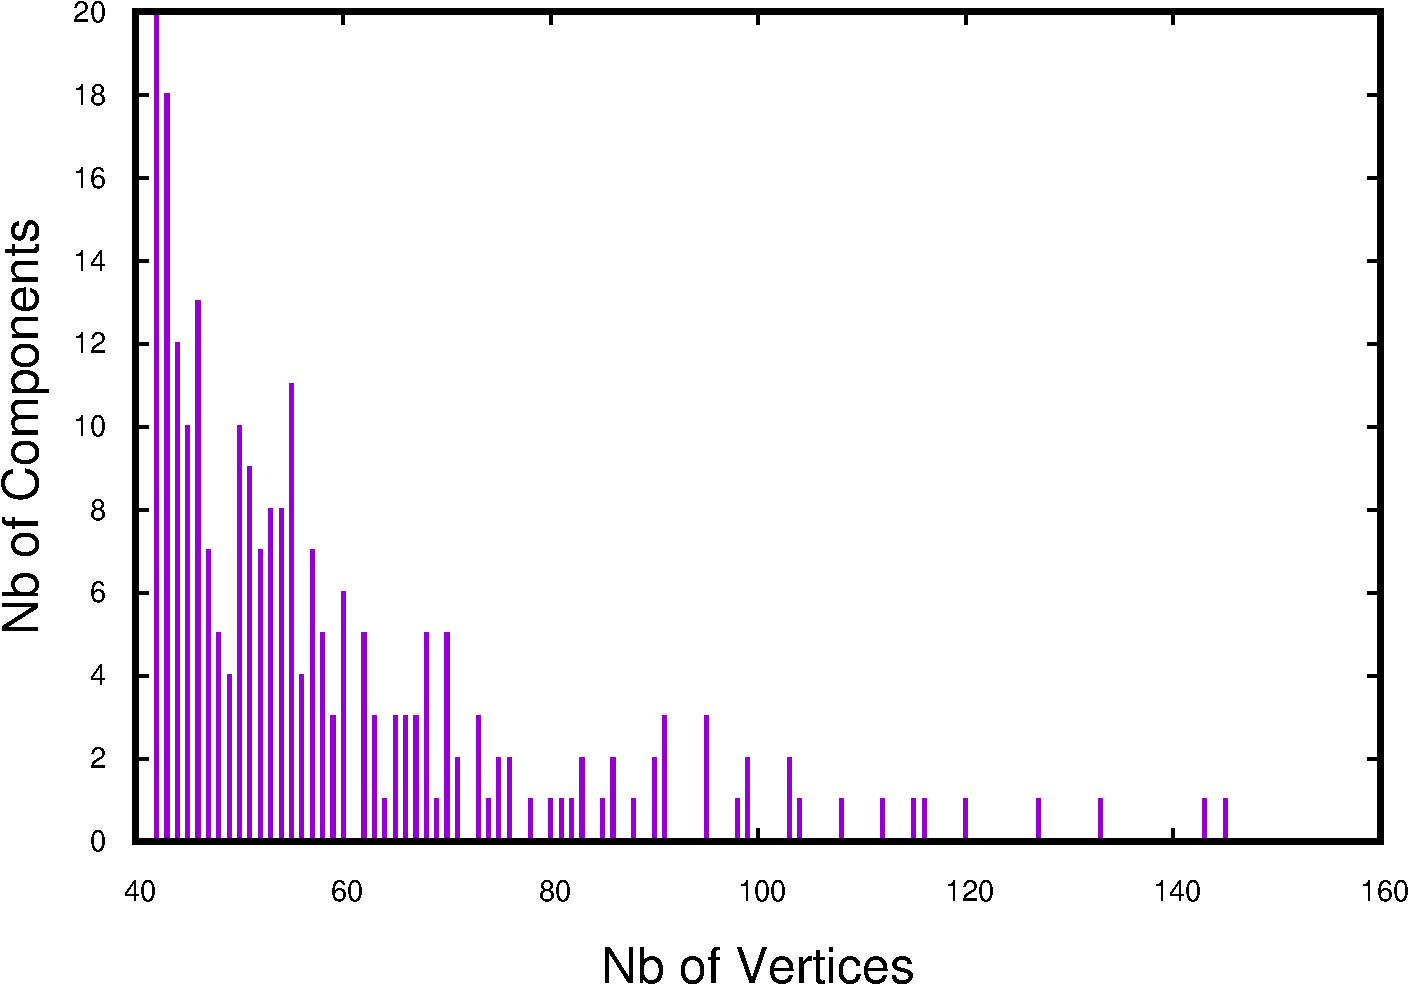
\includegraphics[scale=0.35]{bench/frequency-selected-crop.pdf}
\caption{Components size -- cropped distribution}
\label{fig:cs-selected}
\end{figure}

\begin{table*}[t]
\begin{minipage}[b]{\textwidth}
\caption{Run-time \edited{(in seconds)} for graph $G$}
\label{tab:graph1}
{\small
\centering
\begin{tabular}{||c||c|c|c|c||c|c|c|c||c|c|c|c||c|c|c|c|}
\hline
\textbf{Threads}	&\cellcolor{black!10}BC-4&	\cellcolor{black!10}BC-8	&\cellcolor{black!10}BC-16	&\cellcolor{black!10}BC-32&	\cellcolor{black!10}C-4	&\cellcolor{black!10}C-8&	\cellcolor{black!10}C-16&	\cellcolor{black!10}C-32&	\cellcolor{black!10}D-4&	\cellcolor{black!10}D-8	&\cellcolor{black!10}D-16&\cellcolor{black!10}	D-32&	\cellcolor{black!10}R-4	&\cellcolor{black!10}R-8&	\cellcolor{black!10}R-16&	\cellcolor{black!10}R-32 \\ \hline \hline
64&		27	&17	&22	&41	&53	&34	&32	&52	&26	&15	&20	&41	&23	&17	&20	&39			\\ \hline					
32&		24	&17	&19	&37	&52	&33	&31	&49	&20	&16	&18	&36	&20	&19	&19	&36	\\ \hline
16&		24	&18	&22	&39	&53	&35	&37	&54	&21	&16	&19	&37	&19	&16	&20&37	\\ \hline
8	&	25	&25	&30	&54	&55	&50	&56	&80	&21	&21	&26	&51	&20	&20	&26	&50	\\ \hline
4	&	41	&41	&53	&97	&87	&86	&98	&138	&33	&33	&45	&89	&30	&31	&44	&90	\\ \hline
2&		82	&84	&108	&206	&165	&165	&189	&287	&65	&66	&92	&188	&55	&62	&87	&186	\\ \hline
1&		161	&167	&219	&423	&312	&320	&369	&543	&124	&127	&187	&384	&104	&114	&174	&344	\\ \hline
\end{tabular}
}
\end{minipage}
\end{table*}


\begin{table*}[t]
\begin{minipage}[b]{\textwidth}
\caption{Run-time \edited{(in seconds)} for graph $G_2$}
\label{tab:graph2}
{\small
\begin{tabular}{||c||c|c|c|c||c|c|c|c||c|c|c|c||c|c|c|c|}
\hline
\textbf{Threads}	&\cellcolor{black!10}BC-4&	\cellcolor{black!10}BC-8	&\cellcolor{black!10}BC-16	&\cellcolor{black!10}BC-32&	\cellcolor{black!10}C-4	&\cellcolor{black!10}C-8&	\cellcolor{black!10}C-16&	\cellcolor{black!10}C-32&	\cellcolor{black!10}D-4&	\cellcolor{black!10}D-8	&\cellcolor{black!10}D-16&\cellcolor{black!10}	D-32&	\cellcolor{black!10}R-4	&\cellcolor{black!10}R-8&	\cellcolor{black!10}R-16&	\cellcolor{black!10}R-32 \\ \hline \hline
64		&127	&71	&48	&55	&119	&64	&60	&76	&108	&58	&45	&53	&45	&32	&31	&50		 \\ \hline		
32		&120	&59	&45	&49	&116	&68	&56	&71	&108	&57	&42	&47	&40	&29	&29	&45		 \\ \hline			
16		&128	&66	&39	&52	&115	&66	&65	&79	&112	&57	&36	&50	&41	&33	&30	&46 \\ \hline				
8		&123	&66	&56	&77	&120	&97	&98	&121	&106	&54	&46	&68	&40	&34	&39	&63	 \\ \hline			
4		&164	&104	&101	&142	&210	&191	&185	&223	&134	&83	&80	&119	&60	&57	&69	&113	 \\ \hline			
2		&263	&203	&207	&292	&416	&353	&366	&462	&209	&159	&153	&239	&111	&110	&131	&224	 \\ \hline		
1		&452&357	&371	&525	&761	&804	&793	&969	&355	&281	&286	&434	&196	&201	&230	&402 \\ \hline		
\end{tabular}
}
\end{minipage}
\end{table*}

\begin{table*}[t]
\begin{minipage}[b]{\textwidth}
\caption{Run-time \edited{(in seconds)} for graph $G_4$}
\label{tab:graph4}
{\small
\begin{tabular}{||c||c|c|c|c||c|c|c|c||c|c|c|c||c|c|c|c|}
\hline
\textbf{Threads}	&\cellcolor{black!10}BC-4&	\cellcolor{black!10}BC-8	&\cellcolor{black!10}BC-16	&\cellcolor{black!10}BC-32&	\cellcolor{black!10}C-4	&\cellcolor{black!10}C-8&	\cellcolor{black!10}C-16&	\cellcolor{black!10}C-32&	\cellcolor{black!10}D-4&	\cellcolor{black!10}D-8	&\cellcolor{black!10}D-16&\cellcolor{black!10}	D-32&	\cellcolor{black!10}R-4	&\cellcolor{black!10}R-8&	\cellcolor{black!10}R-16&	\cellcolor{black!10}R-32 \\ \hline \hline
64 &		525&	317	&171&	117	&411	&179&	127	&123	&430	&220	&134	&104&	133&	79&	70	&87	 \\ \hline		
32	&	491&	274	&153	&99	&387	&202	&123	&121 &449	&243&	149&	100	&122	&101&	64&	75\\ \hline
16	&	473	&311	&133	&96	&401	&184	&127	&137 &457	&236	&113	&77	&130	&86	&62	&78 \\ \hline
8	&	557&	250	&132	&126	&387	&234	&204	&212 &452	&222	&113	&105	&119&	93	&75	&93 \\ \hline
4		&750&	333	&221	&234	&612	&431	&374	&398 &601	&274 &168	&190	&151	&126&	120	&163 \\ \hline
2		&1041 &526 &430 &467	&1042	&791	&736	&793 &888	&436	&344	&395	&273	&235	&237	&337 \\ \hline
1		&1626&902&879 &1021 &2156 &1784 &1577 &1754 &1584 &905 &730 &783& 533 &458 &456 &647 \\ \hline
\end{tabular}
}
\end{minipage}
\end{table*}

\begin{figure}
\centering
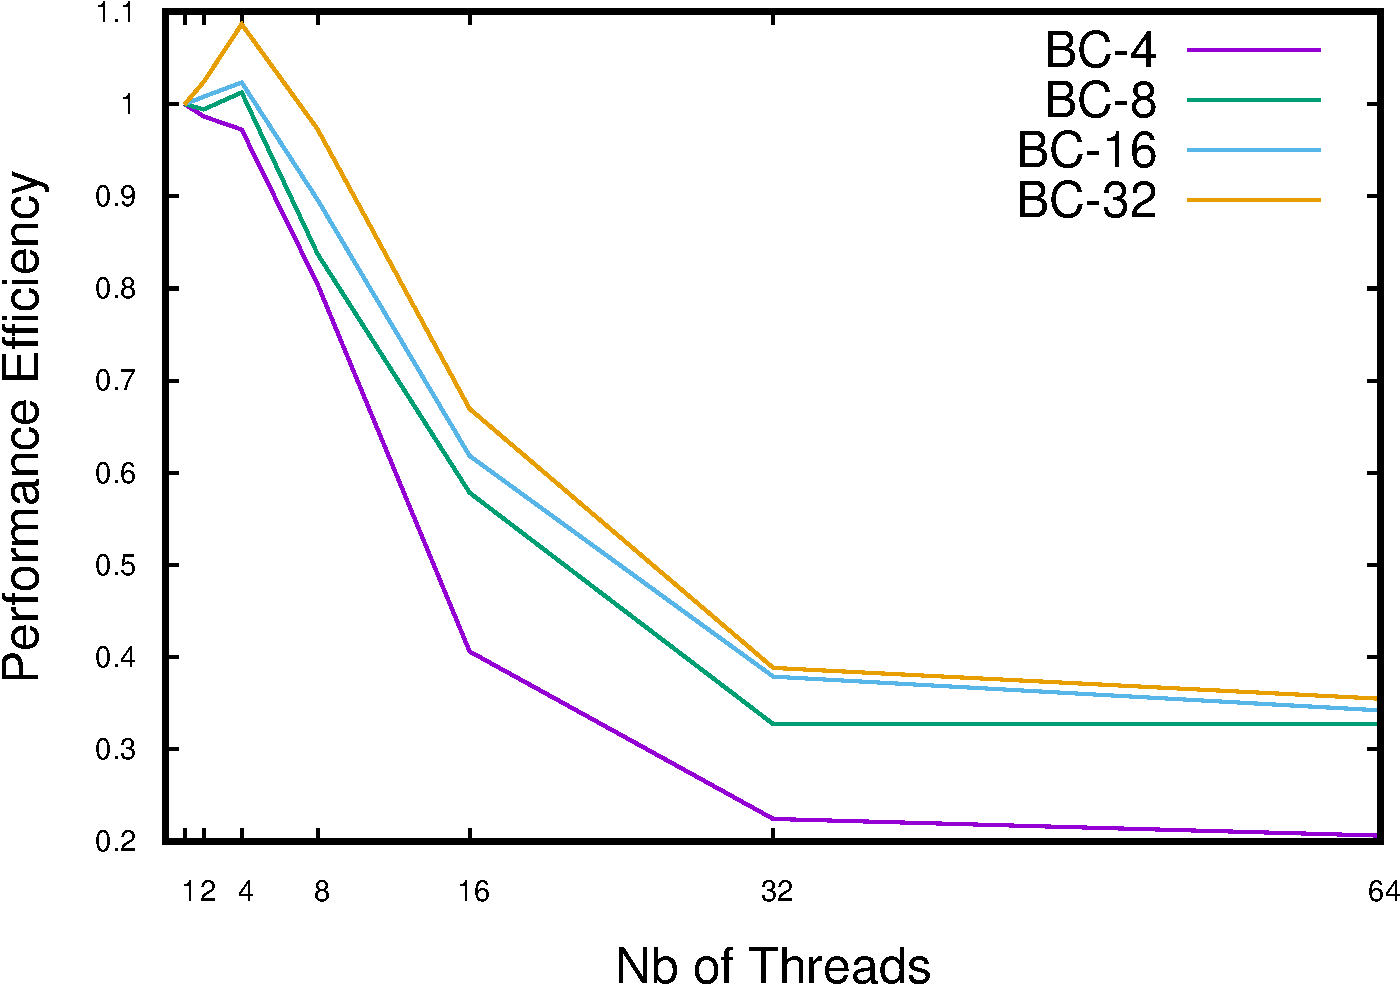
\includegraphics[scale=0.35]{bench/bench-efficiency/efficiency-bc-1-crop.pdf}
\caption{Efficiency for the load based (BC) scenario and graph $G$}
\label{fig:effbc1}
\end{figure}

\begin{figure}
\centering
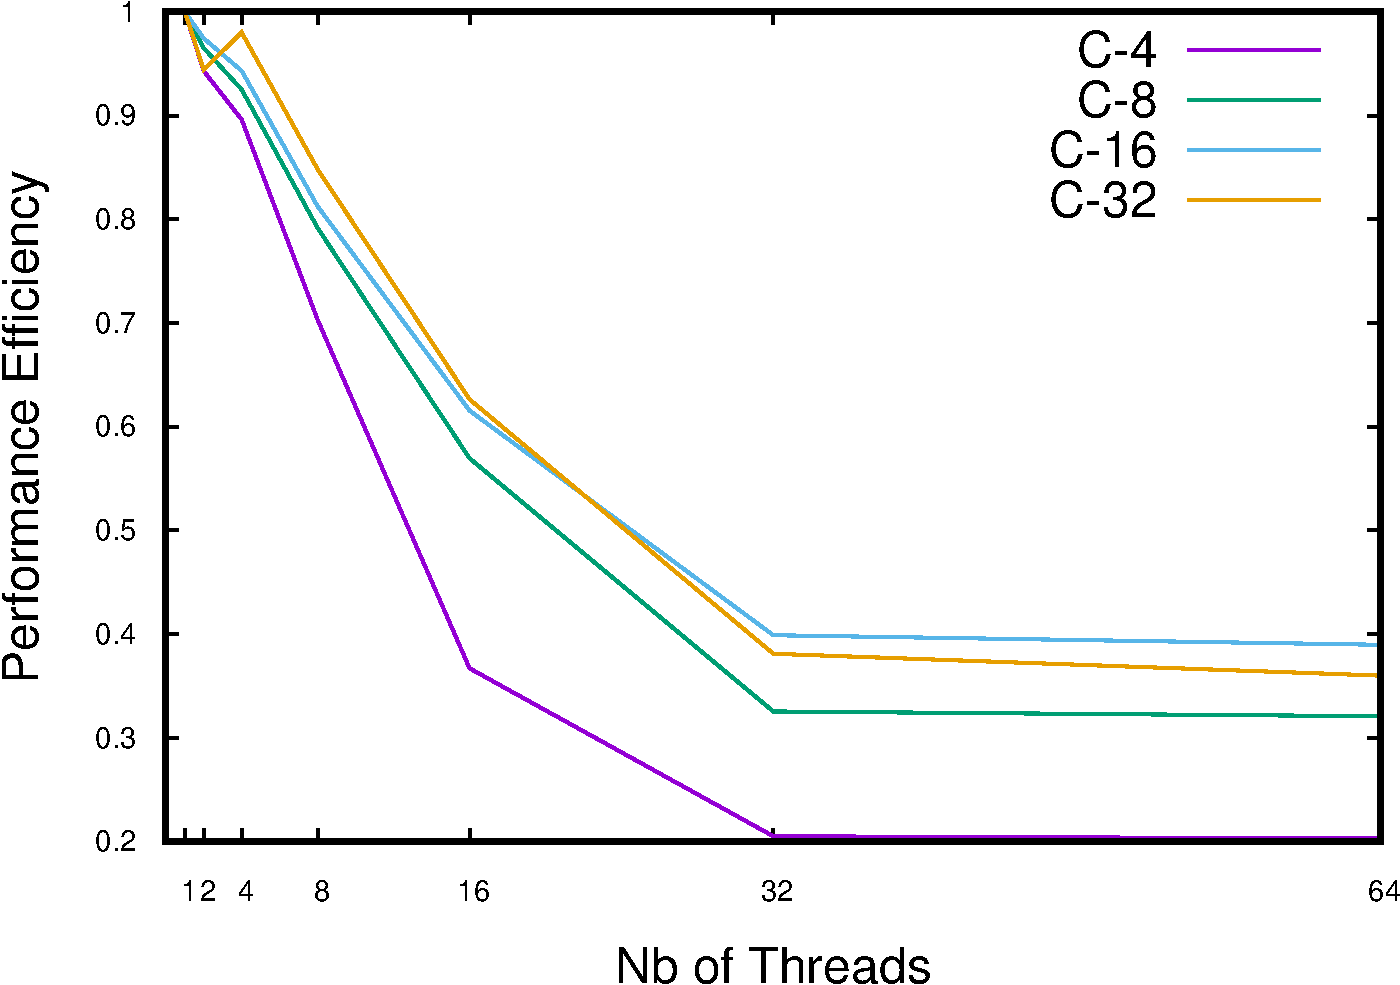
\includegraphics[scale=0.35]{bench/bench-efficiency/efficiency-c-1-crop.pdf}
\caption{Efficiency for the cascading (C) scenario and graph $G$}
\label{fig:effc1}
\end{figure}

\begin{figure}
\centering
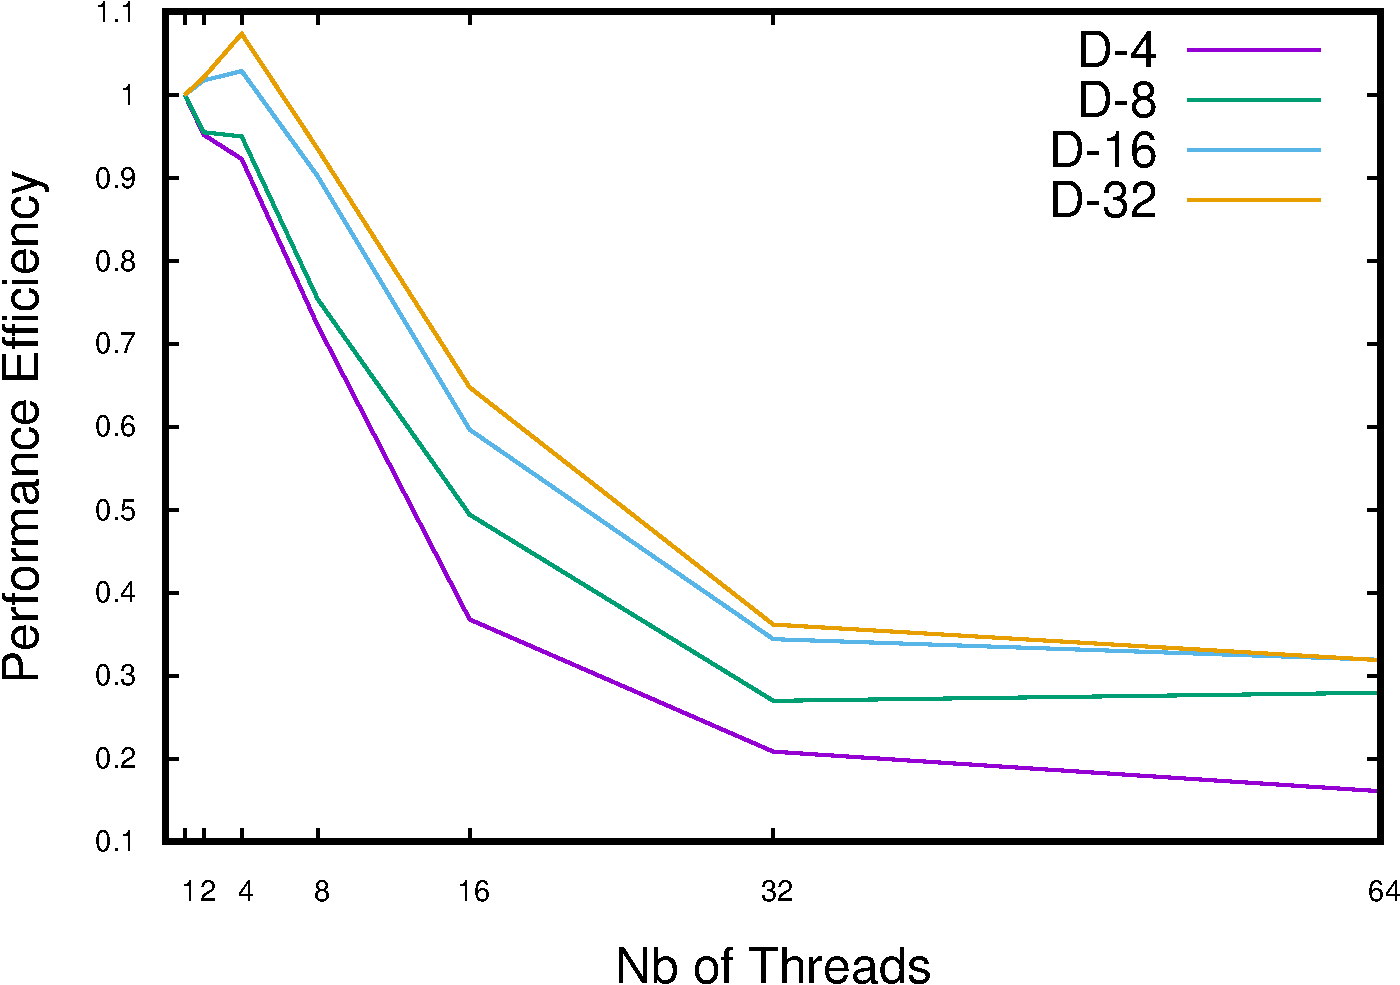
\includegraphics[scale=0.35]{bench/bench-efficiency/efficiency-d-1-crop.pdf}
\caption{Efficiency for the degree-based (D) scenario and graph $G$}
\label{fig:effd1}
\end{figure}


\begin{figure}
\centering
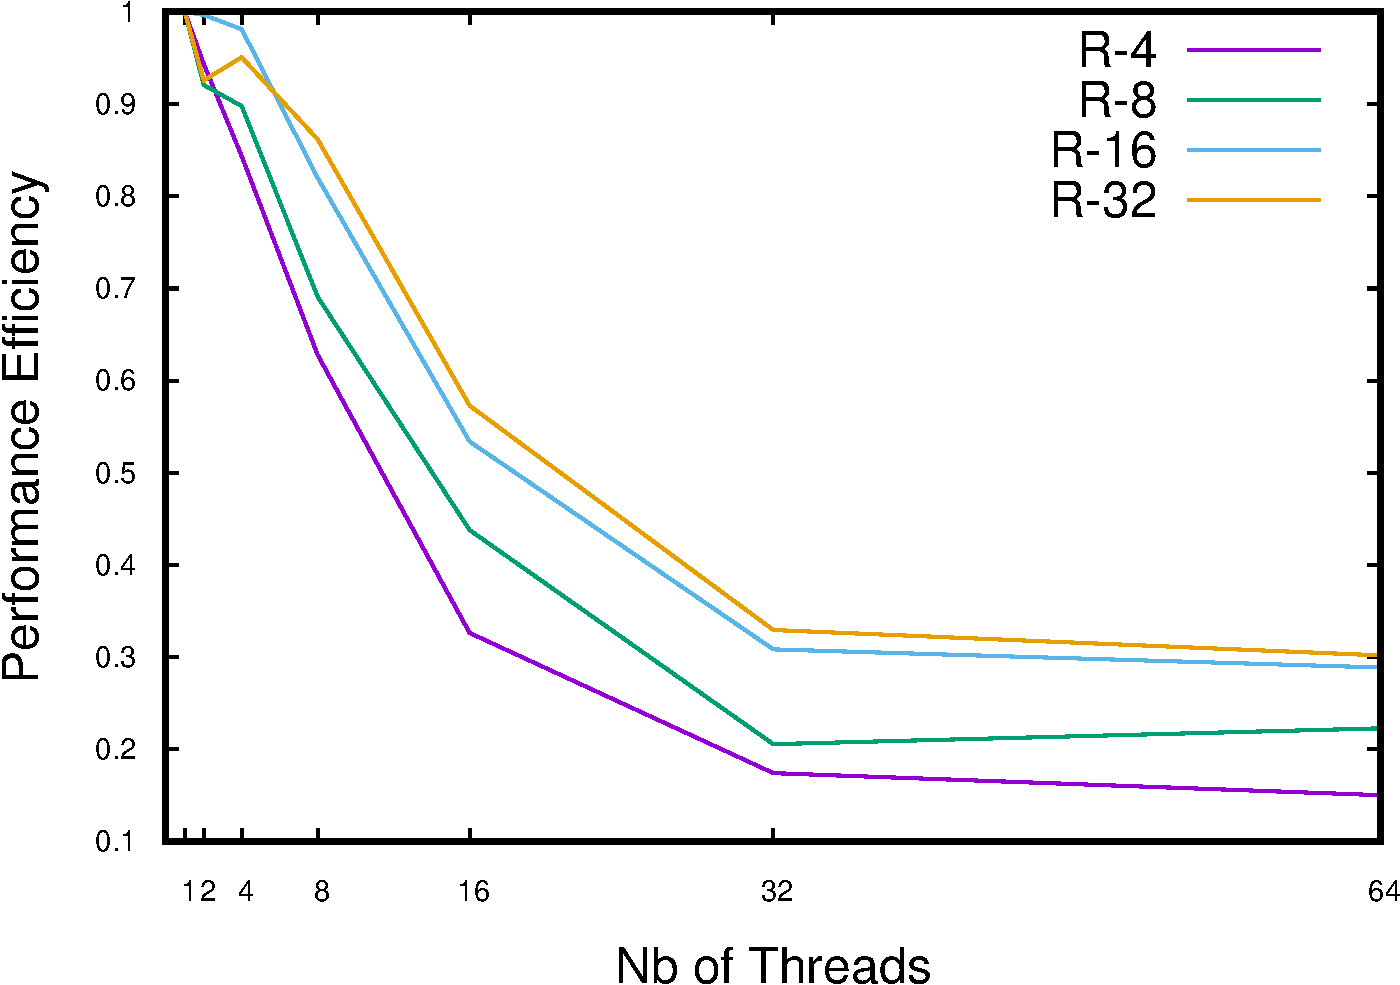
\includegraphics[scale=0.35]{bench/bench-efficiency/efficiency-r-1-crop.pdf}
\caption{Efficiency for the random (R) scenario and graph $G$}
\label{fig:effr1}
\end{figure}

\begin{figure}
\centering
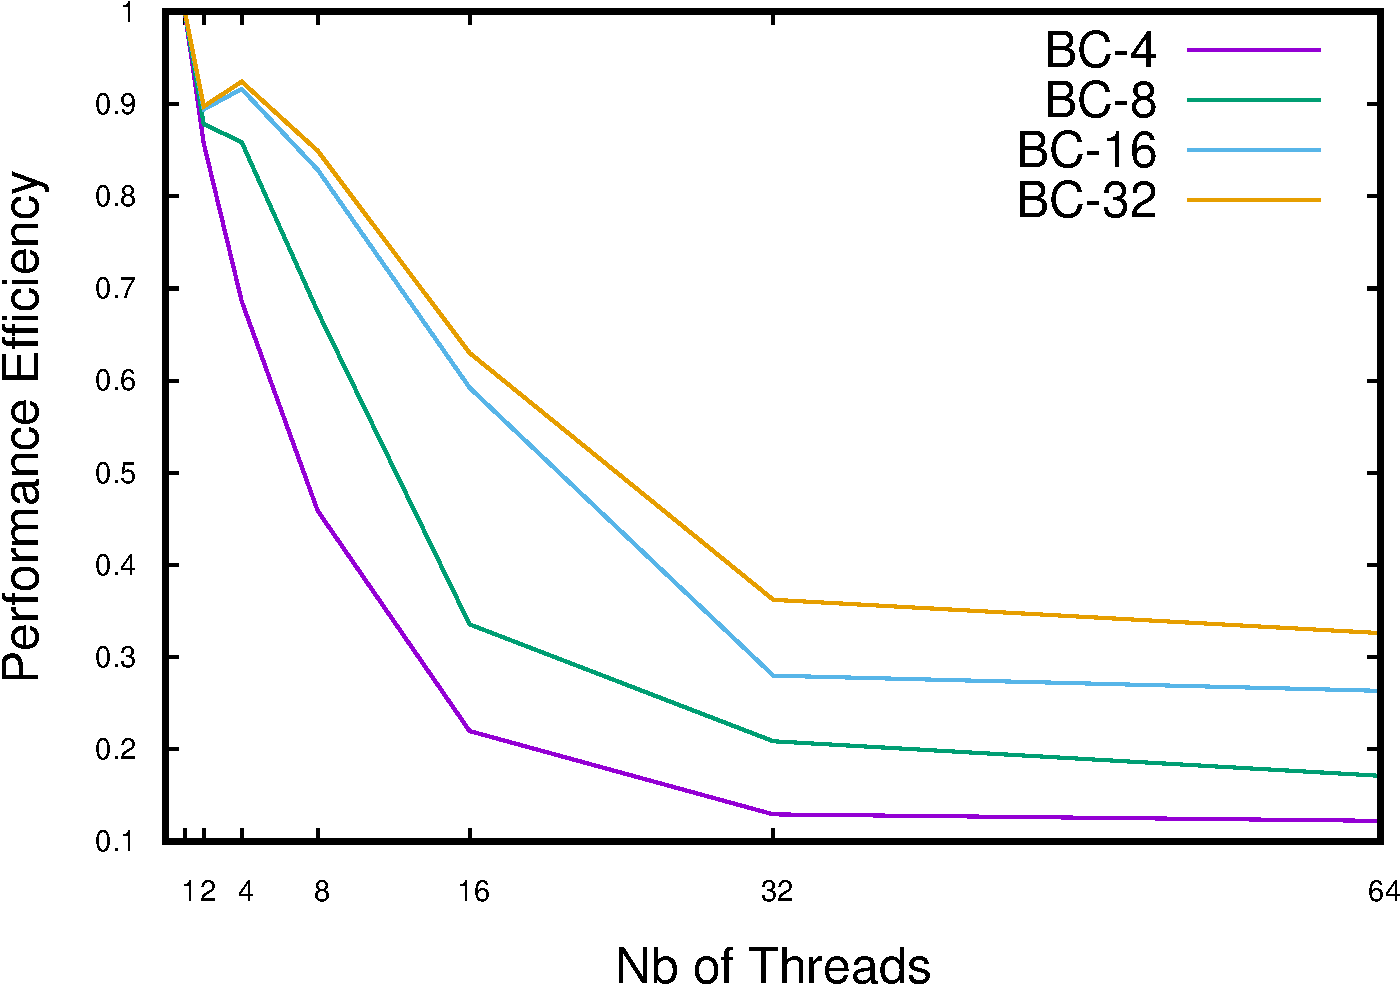
\includegraphics[scale=0.35]{bench/bench-efficiency/efficiency-bc-2-crop.pdf}
\caption{Efficiency for the load based (BC) scenario and graph $G_2$}
\label{fig:effbc2}
\end{figure}

\begin{figure}
\centering
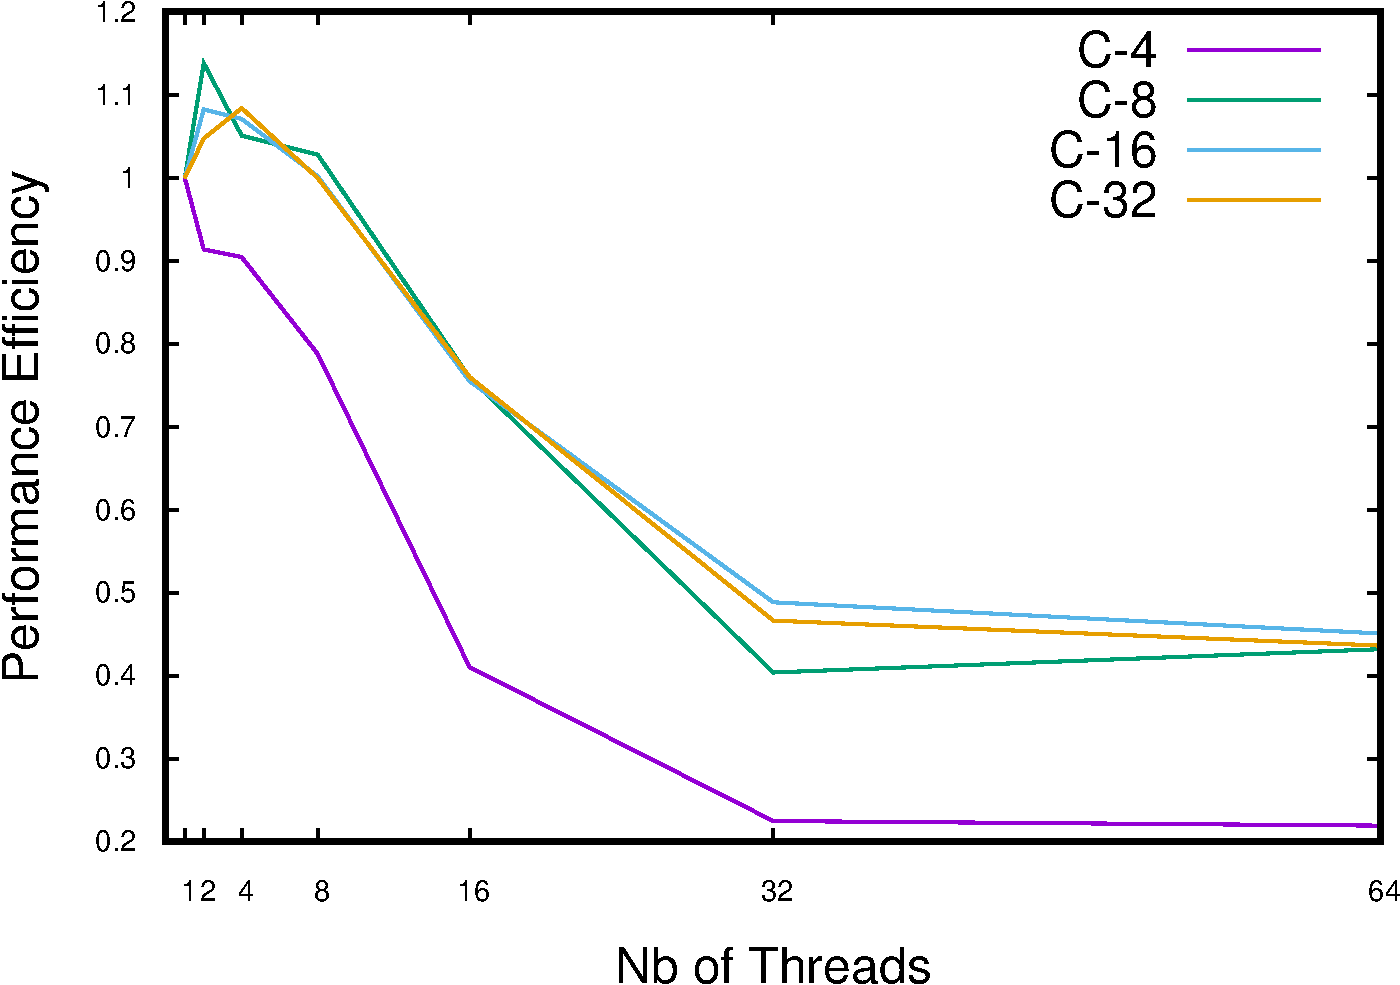
\includegraphics[scale=0.35]{bench/bench-efficiency/efficiency-c-2-crop.pdf}
\caption{Efficiency for the cascading (C) scenario and graph $G_2$}
\label{fig:effc2}
\end{figure}

\begin{figure}
\centering
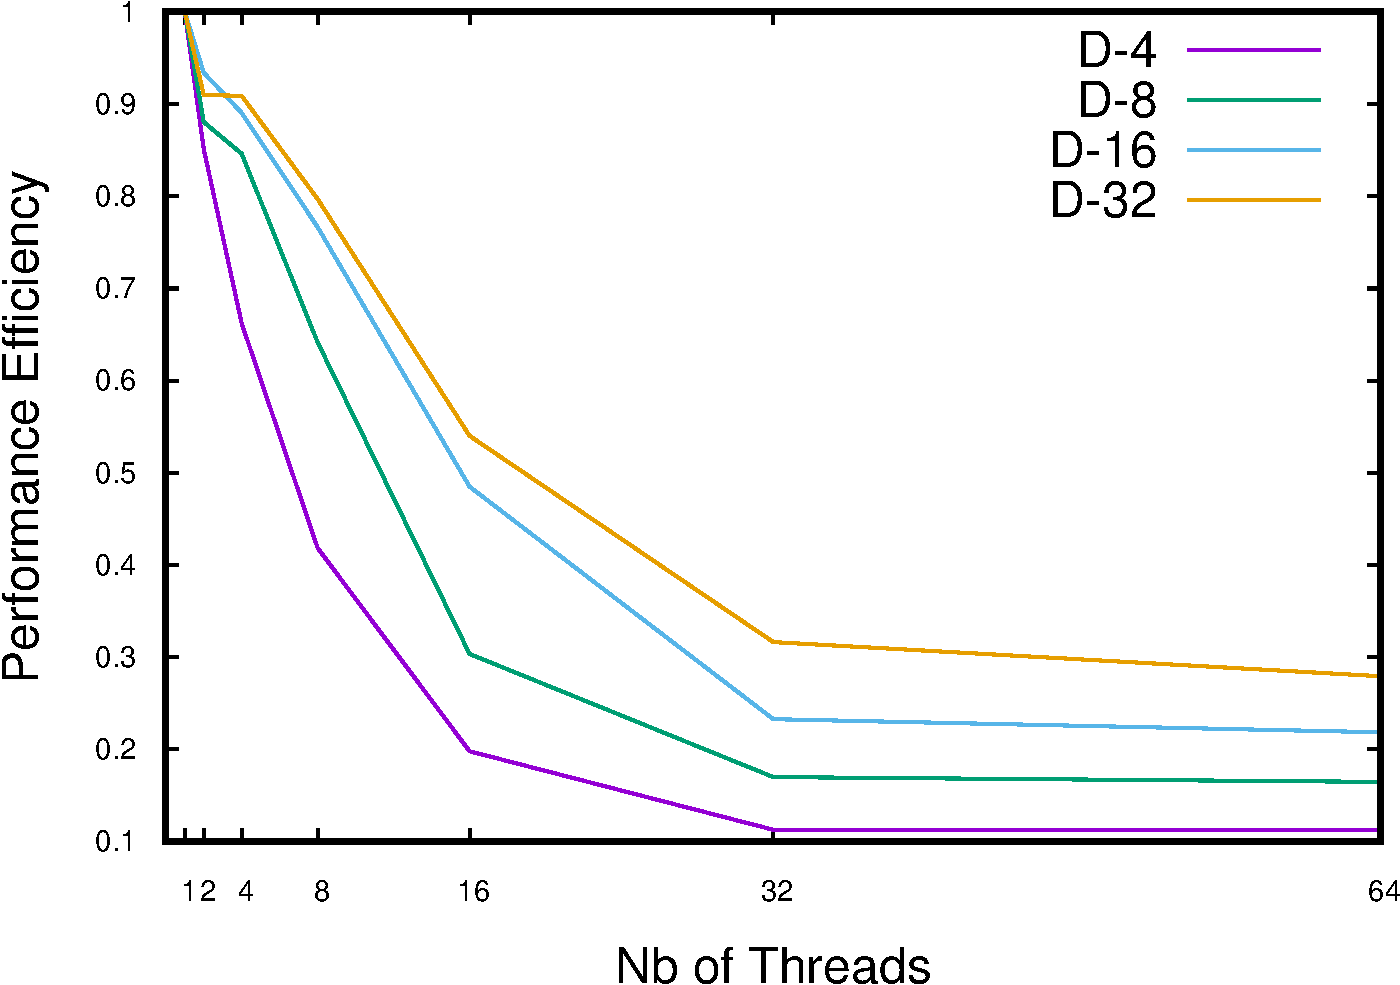
\includegraphics[scale=0.35]{bench/bench-efficiency/efficiency-d-2-crop.pdf}
\caption{Efficiency for the degree-based (D) scenario and graph $G_2$}
\label{fig:effd2}
\end{figure}


\begin{figure}
\centering
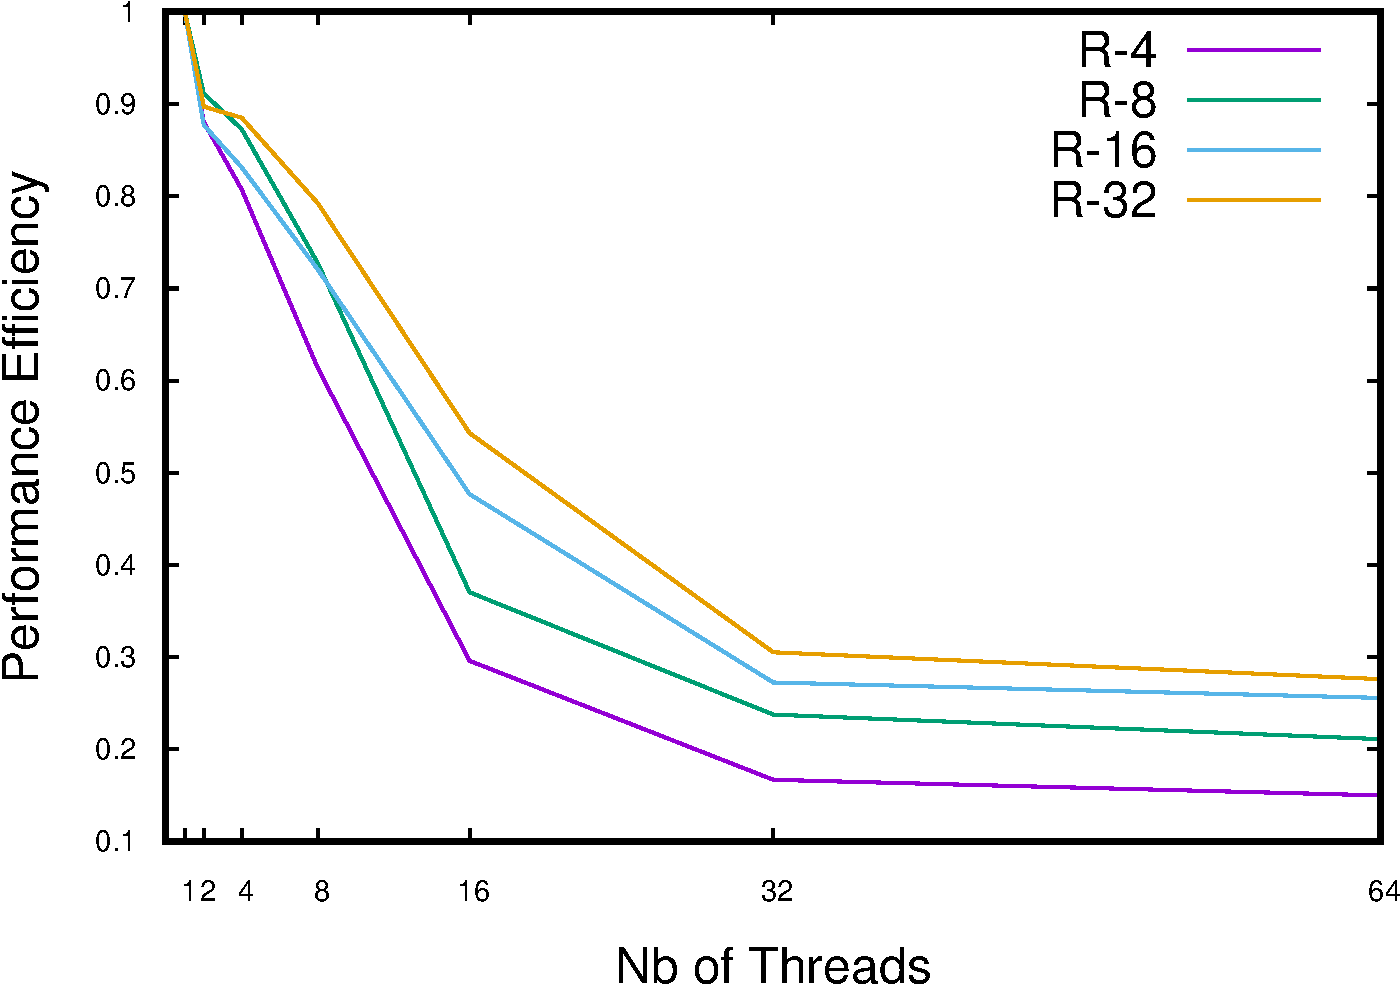
\includegraphics[scale=0.35]{bench/bench-efficiency/efficiency-r-2-crop.pdf}
\caption{Efficiency for the random (R) scenario and graph $G_2$}
\label{fig:effr2}
\end{figure}

\begin{figure}
\centering
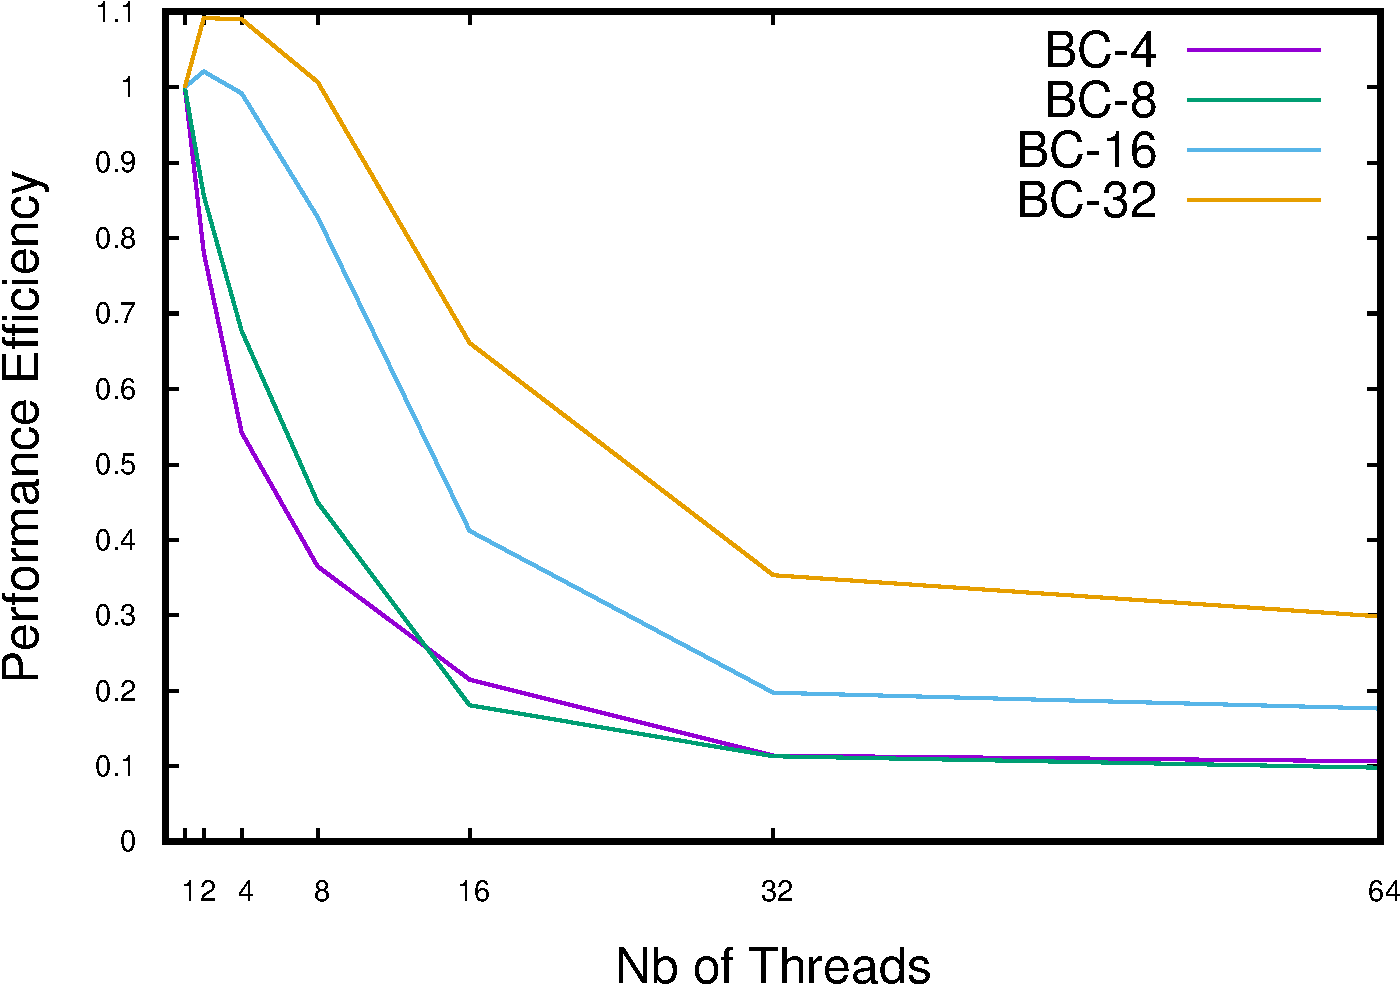
\includegraphics[scale=0.35]{bench/bench-efficiency/efficiency-bc-4-crop.pdf}
\caption{Efficiency for the load based (BC) scenario and graph $G_4$}
\label{fig:effbc4}
\end{figure}

\begin{figure}
\centering
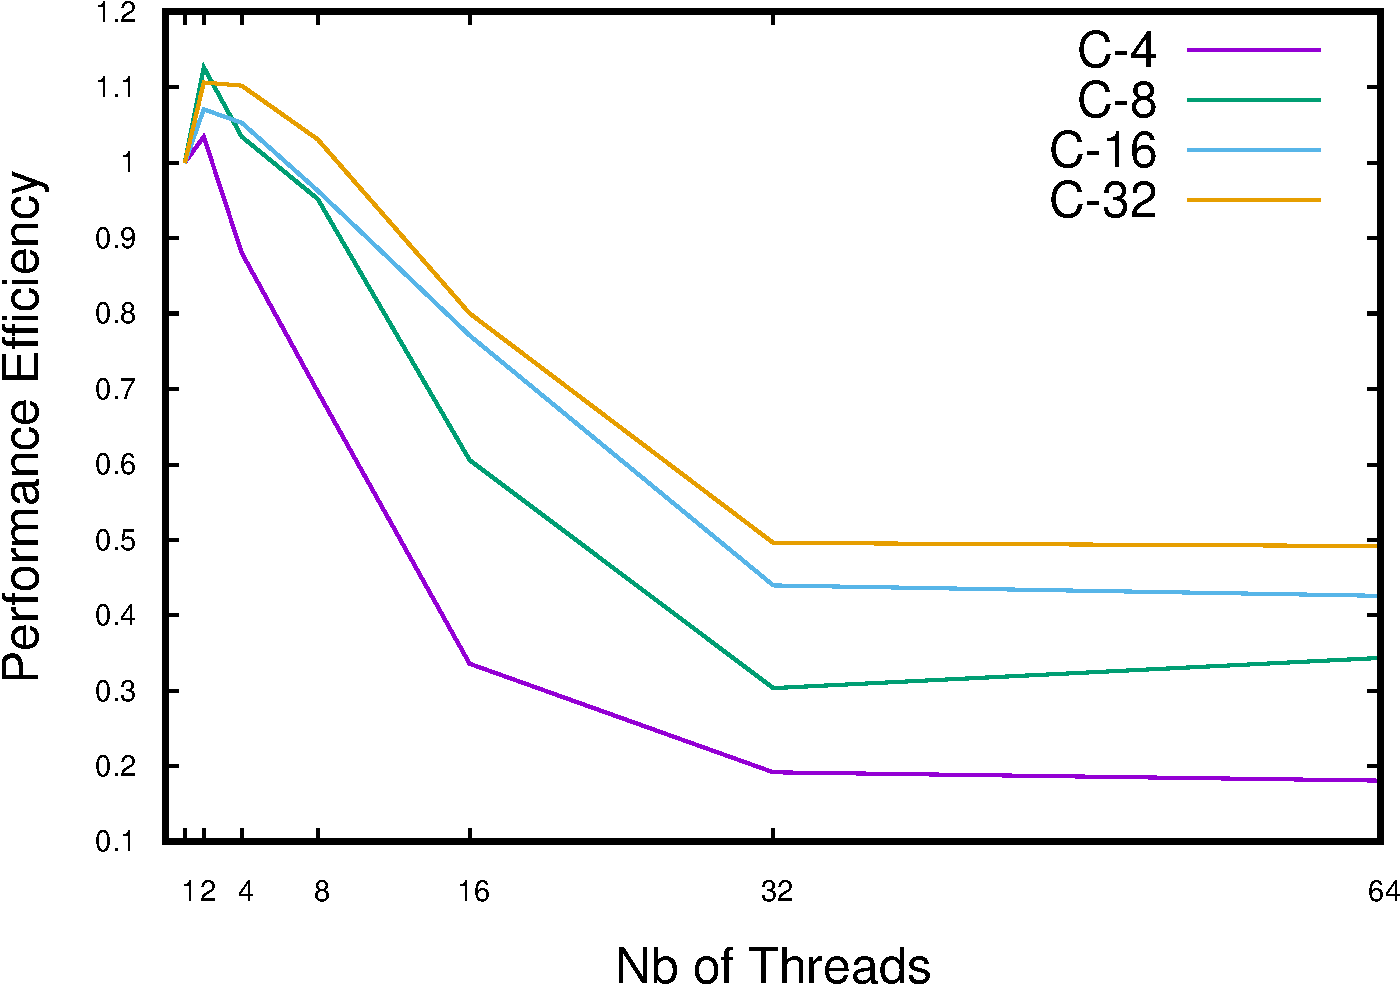
\includegraphics[scale=0.35]{bench/bench-efficiency/efficiency-c-4-crop.pdf}
\caption{Efficiency for the cascading (C) scenario and graph $G_4$}
\label{fig:effc4}
\end{figure}

\begin{figure}
\centering
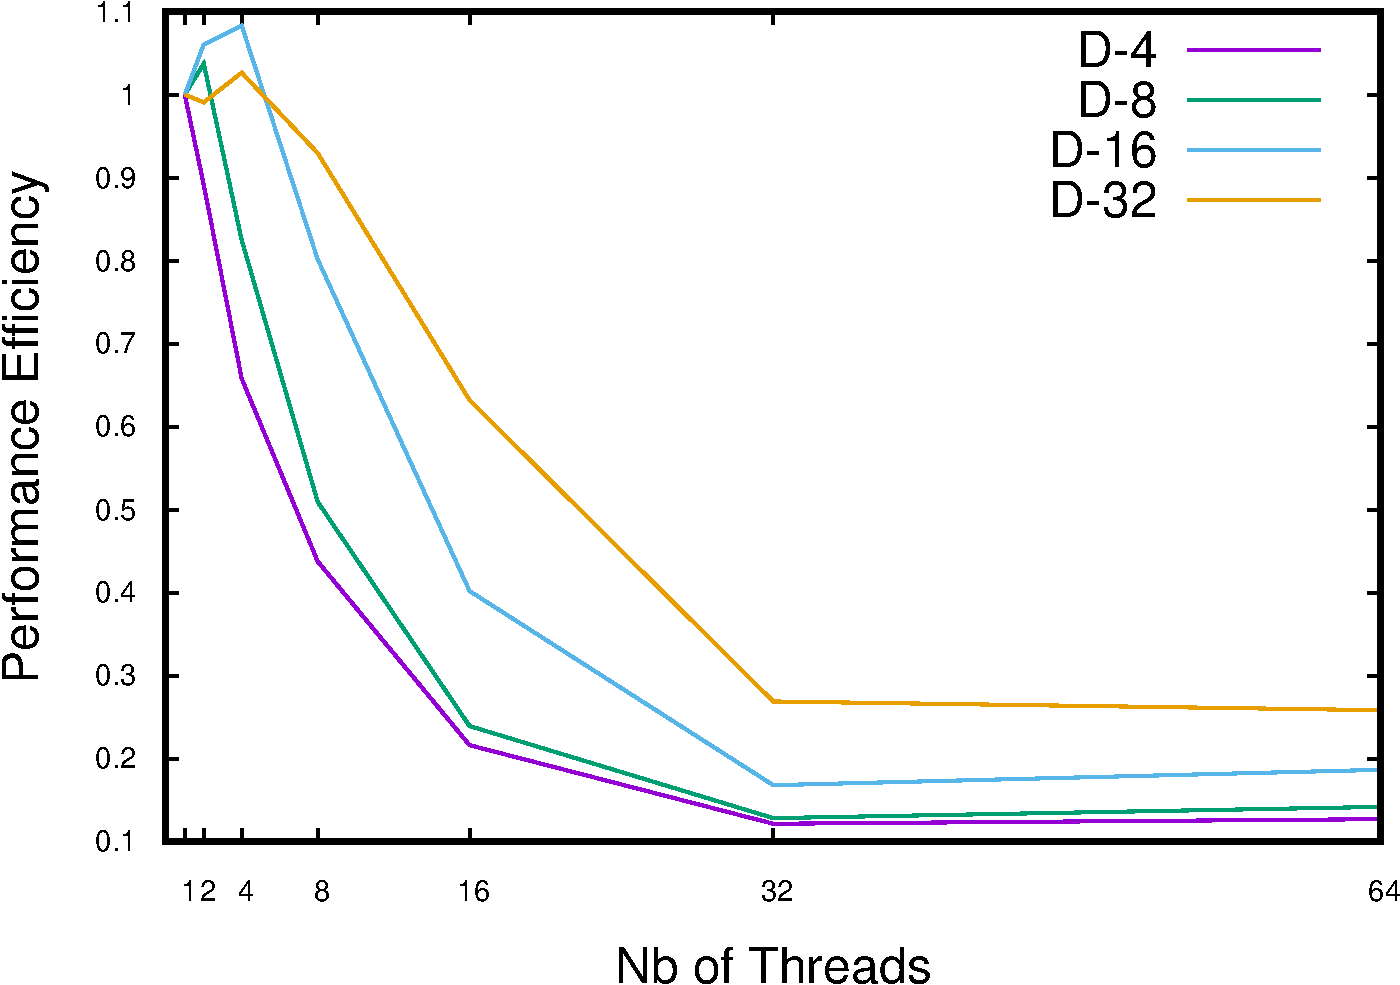
\includegraphics[scale=0.35]{bench/bench-efficiency/efficiency-d-4-crop.pdf}
\caption{Efficiency for the degree-based (D) scenario and graph $G_4$}
\label{fig:effd4}
\end{figure}


\begin{figure}
\centering
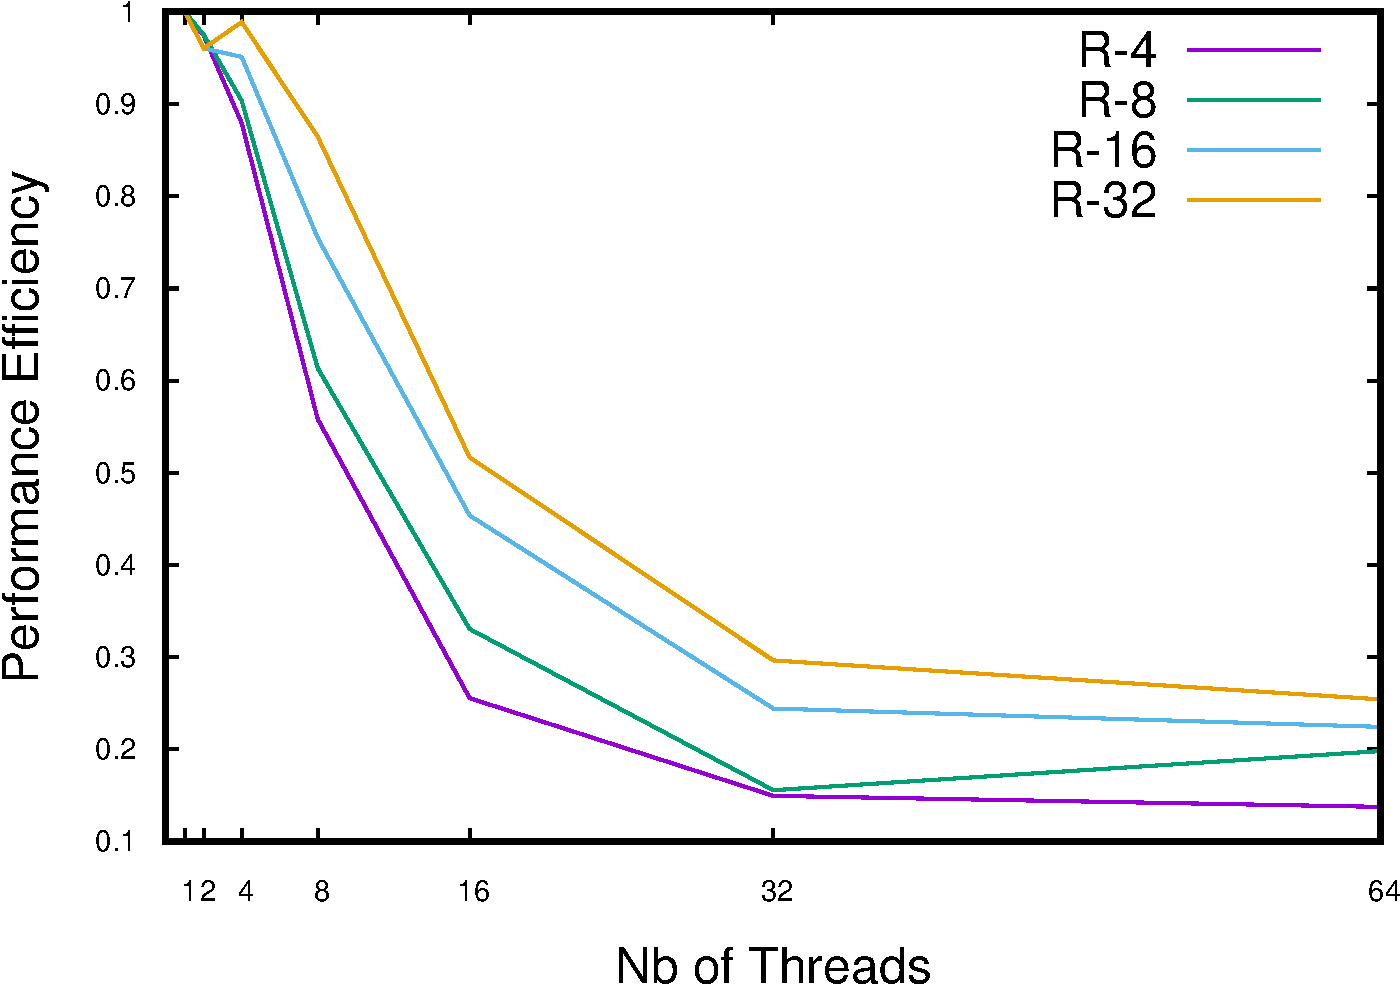
\includegraphics[scale=0.35]{bench/bench-efficiency/efficiency-r-4-crop.pdf}
\caption{Efficiency for the random (R) scenario and graph $G_4$}
\label{fig:effr4}
\end{figure}



\subsection{Spatial analysis}
The spatial correlation analysis shown in Fig. \ref{fig:correlation} reveals a long range correlated case with correlation decaying slowly with distance, particularly, in the linear regime where $C(r) \propto r^{-\gamma} $, $\gamma = 1.13$, which is in agreement with the literature results in \cite{DaqingAl14}.

\begin{figure}
\centering
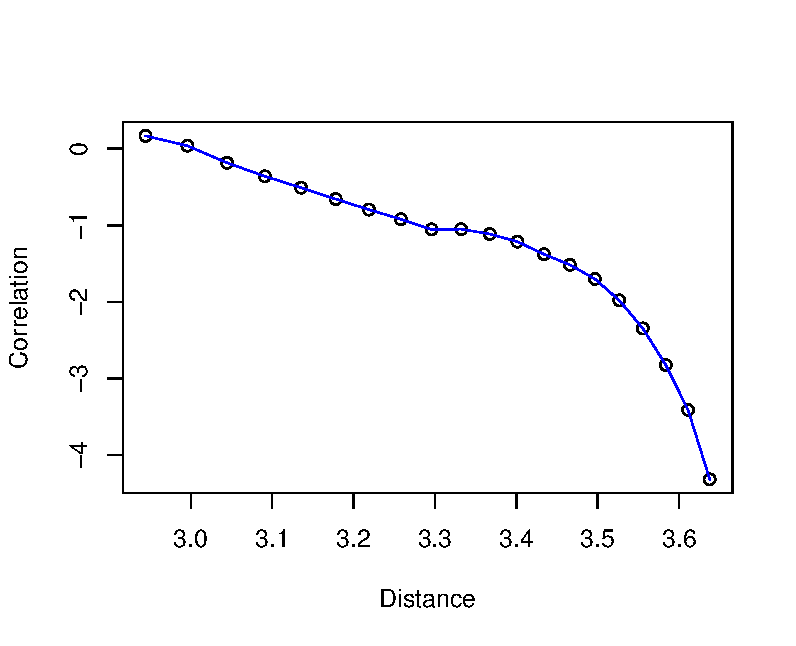
\includegraphics[scale=0.65]{bench/correlation-eps-converted-to.pdf}
\caption{Spatial correlation between nodes in the cascading scenario on a logarithmic scale.}
\label{fig:correlation}
\end{figure}




